\chapter{Návrh riešenia}
V súlade so stanovenými kritériami navrhneme postupnosť krokov úpravy nameraného pohybu dopravného prostriedku. 
Zhotovenú konfigurovateľnú sústavu uplatníme na zariadení senzorovej jednotky za účelom ohlasovania udalostí 
o vybraných pravidelných rysoch signálu. Prihliadať sa bude viac na splnenie úloh v reálnom čase pri
dosiahnuteľnom výkone, v dostupnom pamäťovom priestore, ako na energetickú úsporu. Výmena údajov sa má 
odohrávať zrozumiteľným, širko podporovaným formátom, za obmedzenia nadbytočného sieťového prenosu 
podľa možností.


\section{Špecifikácia požiadaviek}
Zariadenie internetu vecí určené na analýzu vibrácií z prostredia bude realizovať nasledujúce funkčné požiadavky: 
\begin{itemize}[noitemsep,topsep=0pt]
\item Zber trojosovej akcelerácie s nastaviteľnou vzorkovacou frekvenciou a dynamickým rozsahom akcelerometra, v hraniciach danými 
obmedzeniami hardvéru, najmenej však intenzity vyskytujúcej sa pri preprave konvenčnými pozemnými motorovými vozidlami.
\item Spracovanie osí akcelerácie nezávisle s obmedzením výberu aktívnych osí.
\item Vzdialene realizovateľná zmena parametrov jednotlivých stupňov sústavy na úpravu akceleračného signálu v posuvných oknách.
\item Ukladanie nameranej akcelerácie na pamäťovú kartu s ohľadom na najvyššiu dosiahnuteľnú rýchlosť zápisu.
\item Identifikácia významných frekvencií so zachytením ich trvania a amplitúdy podľa aktuálnej 
konfigurácie detekčných algoritmov.
\item Sumarizácia hodnôt akcelerácie po posuvných oknách do popisných štatistík.
\item Odosielanie zachytených udalostí cez spoľahlivé sieťové spojenie za dosiahnutia redukcie množstva produkovaných dát.
\item Poskytnutie možnosti odosielania výsledkov z podstatných medzikrokov spracovania za účelom ich potenciálneho poskytnutia 
ďalším úrovniam senzorovej siete alebo na skupinovú koordináciu meraní z viacerých uzlov. 
\end{itemize}
\bigskip

Z povahy okolností nasadenia firmvéru na relatívne zdrojovo oklieštené Edge zariadenie vyplývajú 
vymenované nie-funkčné požiadavky, prevažne na účinnosť a prenositeľnosť:
\begin{itemize}[noitemsep,topsep=0pt]
\item Firmvér sa zmestí do programovej pamäte s rezervou pre budúce rozširovanie detekčnej funkcionality. 
\item Ľubovoľný scenár spracovania musí prebehnúť v reálnom čase.
\item Odozva detekcie udalostí bude najkratšia možná.
\item Výmena údajov cez sieťový protokol v štandardizovanom formáte hierarchickej štruktúry za najmenšej uskutočniteľnej réžie.
\item Platformová závislosť sa obmedzí na nevyhnuté súčasti systému ako sú hardvérové ovládače a akcelerácia náročných výpočtov.
\end{itemize}

\section{Hardvér senzorovej jednotky}
Navrhované zariadenie bude postavené na platforme mikrokontroléra ESP32 od Espressif. Za relatívne nízkej obstarávacej ceny
ponúka možnosť konektivity na 2,4 GHz s Wifi 802.11 b/g/n alebo Bluetooth 4.2. V porovnaní s podobnými zariadeniami disponuje 
nebývalým výpočtovým výkonom a kapacitou pamätí.

Konkrétne zvolíme dosku FireBeetle osadenú modulom ESP32-WROOM-32D s typickým napájacím napätím 3,3 V a dvoj-jadrovým 
32-bitovým procesorom Xtensa s taktovacou frekvenciou od 80 do 240 MHz. Modul obsahuje až 520 kB zdieľanej SRAM 
pre inštrukcie a dáta. 

Použitý model akcelerometera je súčasťou MEMS inerciálnej meracej jednotky LSM9DS1 zabudovanej na doske
STEVAL-MKI159V1 slúžiacej na adaptáciu do púzdra DIL24. Akcelerometer bude s mikrokontrolérom komunikovať cez
poloduplexnú SPI zbernicu s maximálnou frekvenciou hodín do 10 MHz. Navyše budú zapojené aj vývody prerušení INT1 a INT2
pre upozornenie prekročenia určených prahových úrovní. Blokový diagram zapojenia je na schéme na obr. \ref{schematics:block}.

\begin{figure}[h]
\centering
\begin{subfigure}[b]{0.65\textwidth}
    \centering
    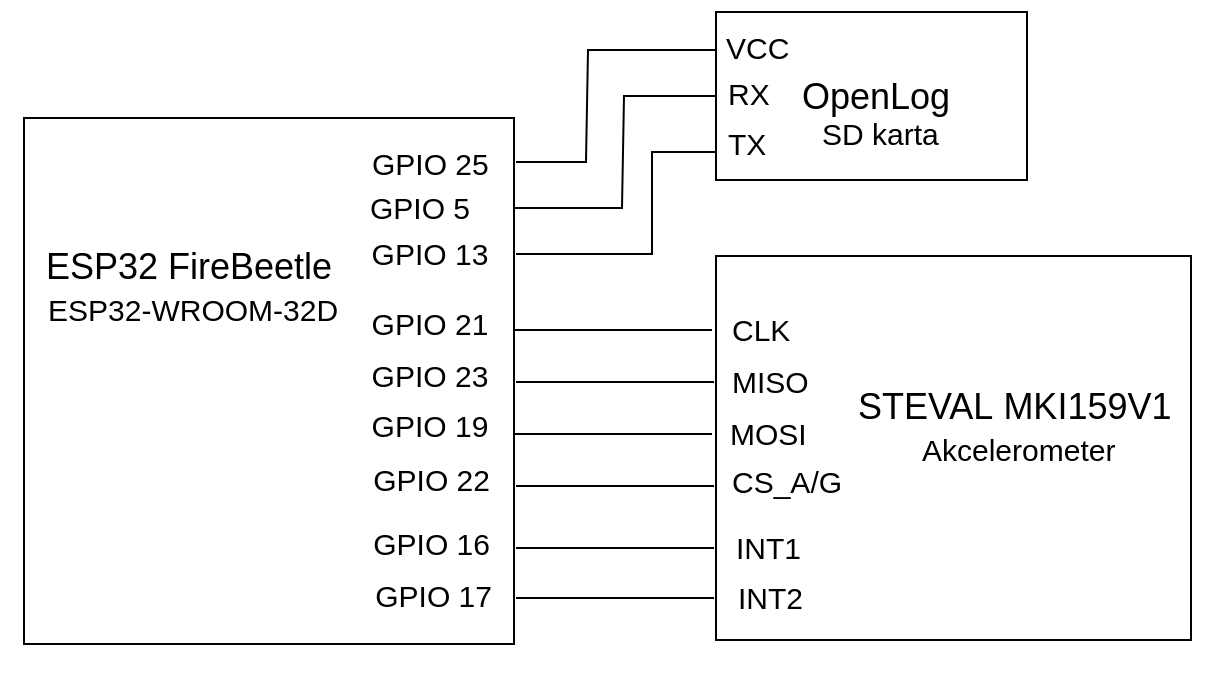
\includegraphics[width=\textwidth]{figures/design/block-circuit-diagram.png}
    \caption{Blokový diagram modulov}
       \label{schematics:block}
\end{subfigure}
\hfill
\begin{subfigure}[b]{0.3\textwidth}
    \centering
    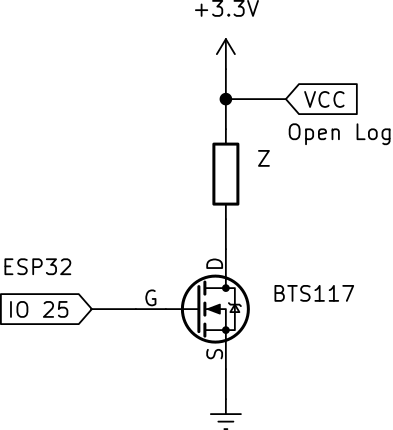
\includegraphics[width=\textwidth]{figures/design/fet.png}
    \caption{Ovládanie napájania OpenLog cez FET}
    \label{schematics:fet}
\end{subfigure}
\label{schematics}
\caption{Schéma zapojenia hardvéru}
\end{figure}
 
Pamäťová Micro SD karta so súborovým systémom FAT32 bude pripojená v module \emph{OpenLog} od Sparkfun, ktorý zaznamená znakový
vstup prijímaný UART zbernicou do textových súborov podľa pravidiel zo súboru \verb|config.txt| alebo povelmi odoslaných 
po zapnutí. Ukladať vzorky na externé médium nie je vždy žiaduce, preto bude napájanie spínané cez pin mikrokontroléra. Vyšší 
prúdový odber než dodá výstup a požadované napätie rovné s napájacím napätím dosky vyžaduje umiestnenie tranzistora riadeného 
poľom N-kanál \emph{BTS117} na premostenie riadiaceho signálu podľa obr. \ref{schematics:fet}.


\section{Architektúra systému}
Celková skladba komponentov systému pozostáva zo súčastí pôsobiacich na mikrokontroléri ESP32
interagujúcimi cez lokálne sériové zbernice s akcelerometrom a zapisovačom. Spracované vektory akcelerácie sú 
odosielané do počítačovej siete prostredníctvom prístupového bodu WiFi aplikačným protokolom MQTT (Message Queue Transport Telemetry)
na server poskytujúci službu MQTT broker správ Eclipse Mosquitto. Odtiaľ sú odoberané témy prešírené klientom metódou publish -- subcribe.
Diagram na obr. \ref{uml:component} zachytáva náhľad na zloženie vymenovaných komponentov. 

\begin{figure}[h]
	\centering
	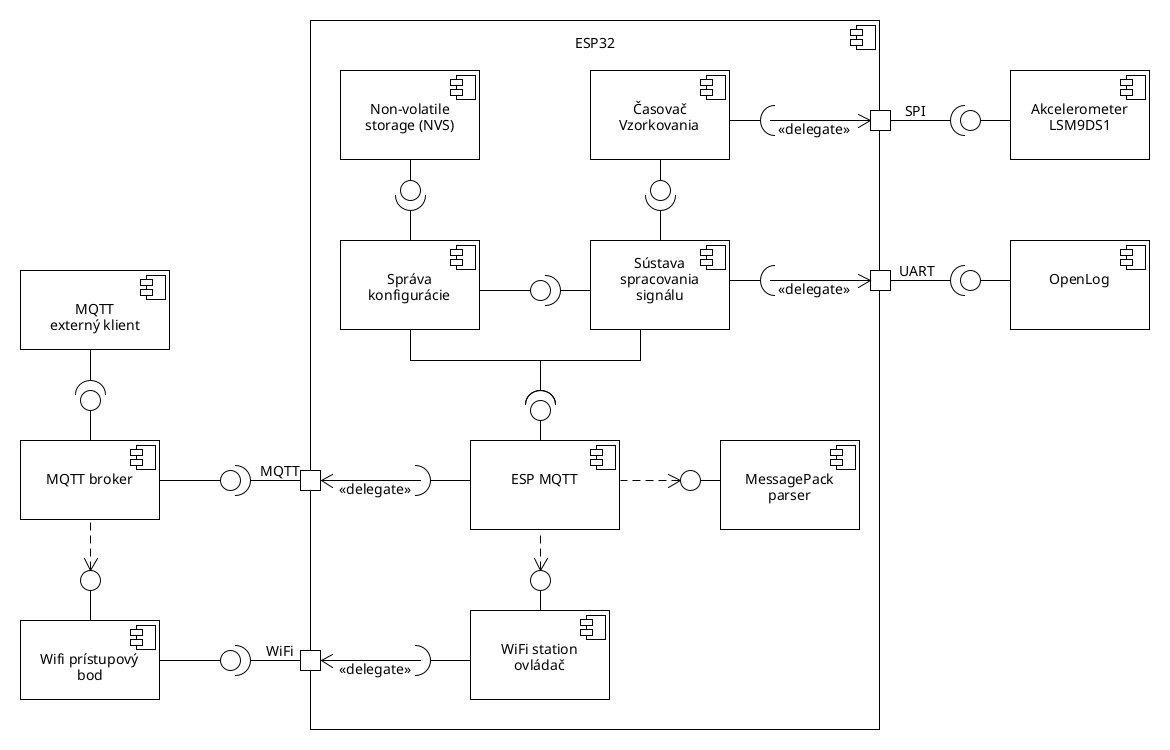
\includegraphics[width=\textwidth]{figures/design/components.png}
	\caption{Komponenty navrhovaného systému}
	\label{uml:component}
\end{figure}

Odčítavanie úrovní z akcelerometra zabezpečuje \textbf{časovač vzorkovania}, ktorý si v pravidelných intervaloch pýta aktuálne 
hodnoty rozhraním periférneho adaptéra pre prístup ku SPI zbernici. Po vypršaní vzorkovacej periódy je zavolaná obsluha prerušenia, ktorá 
odblokuje vlákno úlohy na synchrónne načítanie okamžitého vektora zrýchlenia konvertovaného z číslicovej úrovne prevodníka na metre za 
sekundu na druhú. 

Zachytené hodnoty sú preposlané cez thread-safe fronty analyzátora signálu zvlásť pre každú priestorovú os akcelerácie. 
V prípade nutnosti zachytávať časový priebeh s príslušných podvzorkovaním sa vektor umiestni do frontu smerom ku vláknu loggera. 
Postup vzorkovania ilustruje sekvenčný diagram na obr. \ref{uml:sequence}.

\textbf{Pipeline spracovania signálu} rozdeľuje vzorky do prelínajúcich sa posuvných okien, počíta z nich štatistiky a vyhľadáva udalosti vo 
frekvenčnom spektre. Nespracované hodnoty sú podľa potreby ukladané na pamäťovú kartu. 

Zmenu a uchovanie parametrov pipelinov pre jednotlivé bloky spracovania zaobstaráva \textbf{správa konfigurácie}. Modifikované nastavenia sú 
medzi spusteniami zachované vo vyhradenej partícií nevolatilnej flash pamäte na záznamy dvojíc v asociatívnej štruktúre. Predvolené 
správanie načítané pre nedostupnosť stavu z flash úložiska určujú konštanty v programovej pamäti.

Binárny serializačný formát Message Pack zaobaluje vzorky, udalosti a konfigurácia posielané na rozličné MQTT témy. Vychádza z 
formátu JSON (JavaScript Object Notation), ale narozdiel od neho sa sústredí na efektívne kódovanie dátových typov. Namiesto prevodu 
číselných údajov do znakového kódovania, napr. Unicode, ponecháva ich pôvodnú binárnu reprezentáciu s špecifikovanou bytovou značkou 
určujúcou typ. Hodnoty vyjadriteľné menším počtom bajtov reprezentuje dokonca v kratšom tvare než podmieňuje ich celkový rozsah.
Rovnako v zoznamoch a slovníkov sa  zaobchádza bez oddelovacích znakov, ktoré nahrádza informáciou o počte údajov. Dĺžka 
položky predchádzajúca zloženými atribútom uľahčuje následné parsovanie.

\begin{figure}[h]
	\centering
	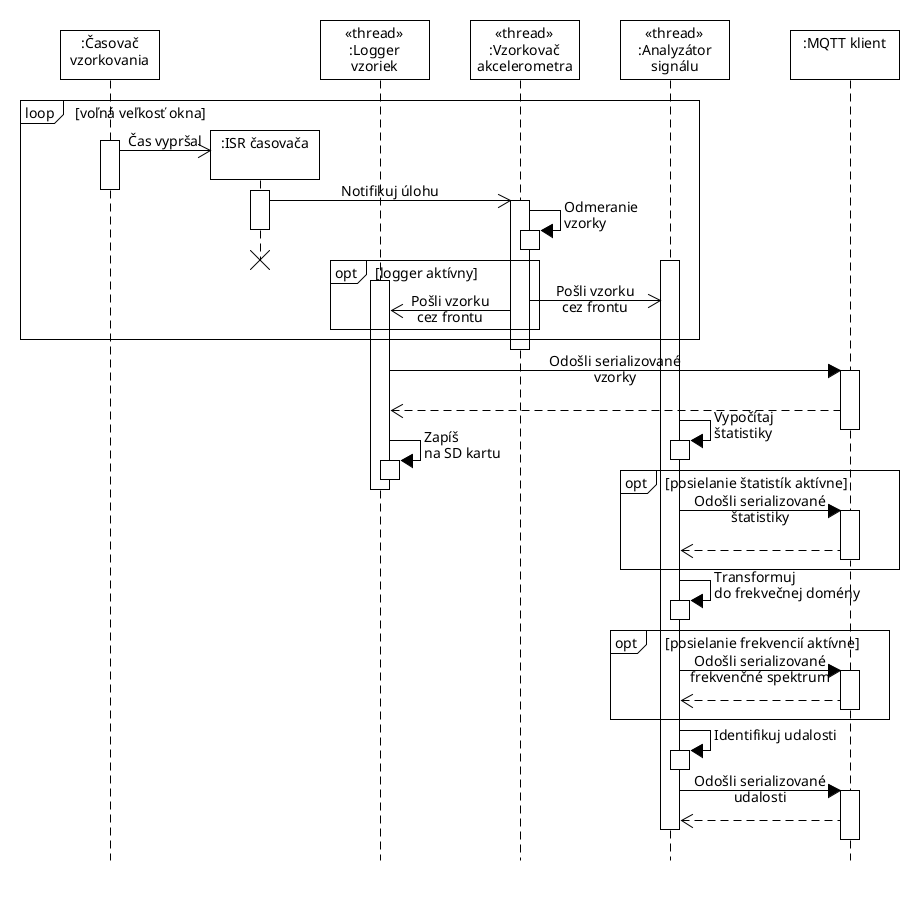
\includegraphics[width=\textwidth]{figures/design/tasks.png}
	\caption{Sekvenčný diagram vzorkovania signálu}
	\label{uml:sequence}
\end{figure}

\section{Funkčné bloky dátovej pipeline}
Poskladaná dátová pipeline sa sústredí primárne na odhalenie pretrvávajúcich spektrálnych zložiek. Úloha jednotlivých 
zakomponovaných blokov spočíva v prevedení pôvodne obdržaných vzoriek podľa globálnych pravidiel definujúcich ich správanie. 

Vo všeobecnosti sa v nej nachádzajú bloky filtrácie, transformácie alebo serializácie signálu. Sústava sa 
vyznačuje modulárnosťou, čiže umožňuje doplnenie dodatočných, ale iba v jednej na seba nadväzujúca
línia naraz, so spoločnou veľkosťou posuvného okna a ich vzájomnému prekryvu. Diagram aktivít na obr. \ref{pipeline}
vizualizuje navrhovaný beh činností na zariadení.

\subsection{Nastaviteľné vlastnosti}
Utváranie charakteru výstupov sa deje hneď na začiatku voľbou nastavení snímača.
Vzťahuje sa na ne vzorkovacia frekvencia časovača, podmieňujúca výstupný dátový tok konštrukčne obmedzený do 952 Hz, 
a dynamický rozsah v rozmedzí do 16g. Keďže sú priestorové osi zrýchlenia analyzované nezávisle vyžadujú sa pre každú ďalšiu
dimenziu systémové prostriedky navyše, ktoré by vyšli navnivoč pokiaľ sú osi korelované alebo sa sleduje pôsobenie v 
známom smere. Možnosť aktivácia len niektorých osí je preto výhodná.

Postupnosť hodnôt je rozkúskovaná podľa dĺžky vyrovnávacej pamäte s počtom slotov čítajúcim dokopy mocninu dvojky
z dôvodu náväznosti na prevod do frekvenčnej domény. Pomer prekryvu okien sa odporúča od 0, čo znamená bez zanechania časti predošlého 
obsahu, do nanajvýš 0.75 výhradne pre úzke oknové funkcie.

Po naplnení miest v opísanej cyklickej fronte sa pristúpi k prenásobeniu bodov s koeficientami oknovej funkcie 
z ponuky: obdĺžnik, Bartlett, Hann, Hamming, Blackman, a následnej Fourierovej alebo kosínusovej transformácii o veľkosti totožnej s dĺžkou 
okna. Z frekvenčných vedierok sa zistí magnitúda v lineárnej alebo decibelovej škále. 
Pred a po transformácii sa môže doplnkovo uplatniť filter vyhladzovania priemerom v časovej ako i vo frekvenčnej doméne.
Opierajú sa o stanovenú veľkosť masky filtra a počet prechodov koľkokrát má byť opakovane aplikovaný.

Identifikácia udalostí pozostáva z binárnej klasifikácie úrovní frekvenčných vedierok podľa prítomnosti lokálneho maxima a
zo zlúčenia súvislého výskytu naprieč dlhším časovým intervalom do udalosti. Klasifikácia sa realizuje 
aktuálne nastaveným algoritmom na hľadanie špičiek podľa kombinácie príslušných číselných parametrov. K dispozícii sú
algoritmy nad prahovou úrovňou, najvyššieho spomedzi susedov, prechodu nulou do záporu alebo horského turistu.

Medzi dôležitými fázami pipeline dochádza podľa povolených modulov na odosielanie správ k odovzdaniu medziproduktov na formátovanie
cez Message Pack a synchrónne publikovanie na MQTT tému. Umožňuje sa poslanie vzoriek po decimácii celočíselným faktorom $\geq 1$, 
požadovaných štatistík z časového priebehu (minimum, maximum, stredná kvadratická odchýlka, priemer, rozptyl, smerodajná odchýlka,
šikmosť, špicatosť, medián, mediánová absolútna odchýlka, medzi-osová korelácia), výsledku frekvenčnej transformácie alebo udalostí 
o zmene významných frekvencií.

\begin{figure}[h]
	\centering
	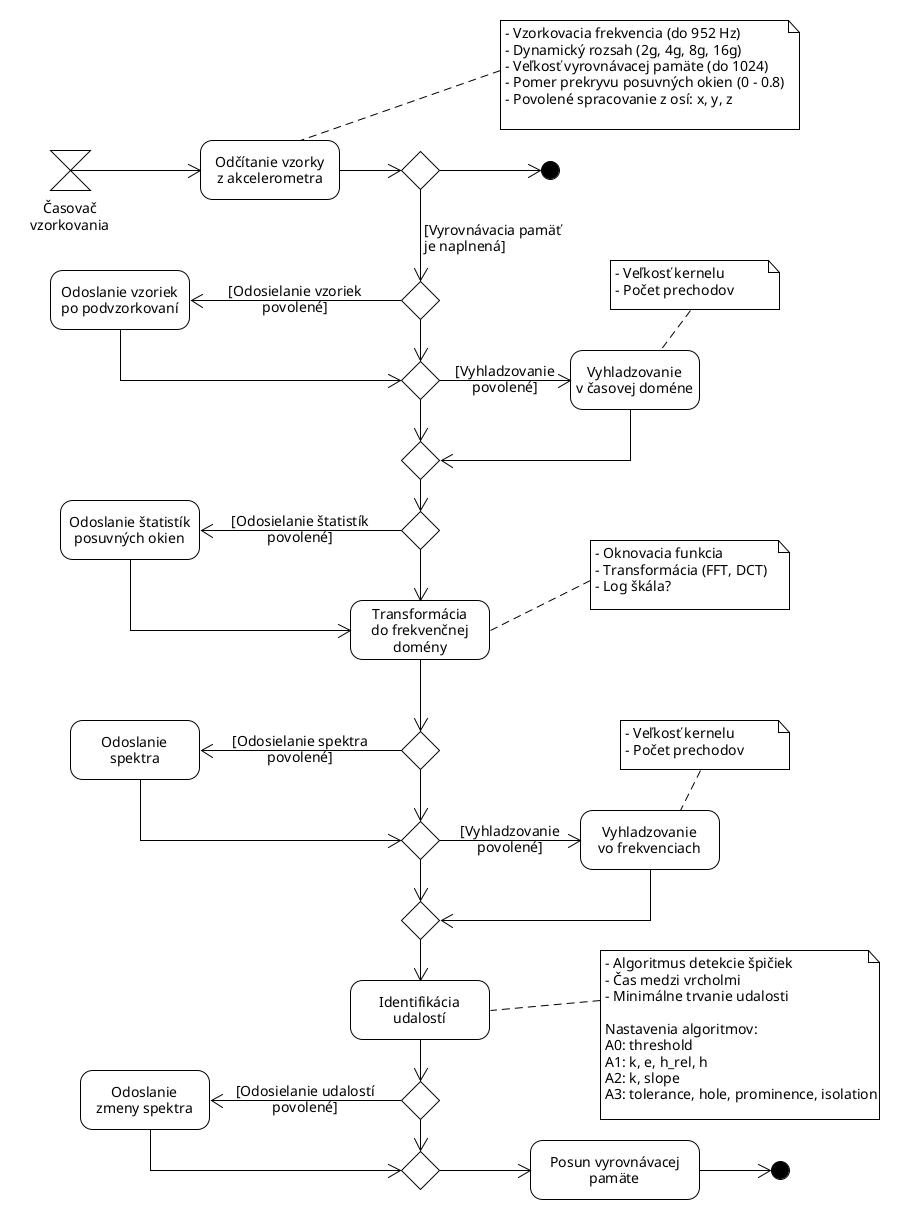
\includegraphics[width=0.9\textwidth]{figures/design/pipeline.png}
	\caption{Postup spracovania zaznamenávaných vibrácií}
	\label{pipeline}
\end{figure}

Reguláciu toku dát a vlastnosti úpravy v blokoch pipeline ovplyvňuje globálna systémová konfigurácia. Obvykle sa nahrá
z nevolatilnej pamäte, ale je umožnené, aby pravidlá boli upraviteľné vzdialene správami vo formáte Message Pack. 
Postup ukazuje diagram na obr. \ref{config-change}.

Zariadenie sa prihlási na odber MQTT témy na zmenu konfigurácie a postačuje, aby tam klient odoslať atribúty, ktoré mieni
modifikovať. Ak sú parametre syntakticky korektné a spadajú do dovoleného číselného intervalu príde k reštartu zariadenia a ich
uplatneniu. V opačnom prípade sa na samostatnú MQTT tému odošle chybová hláška. Vzdialený klient si taktiež dokáže zobraziť 
všetky momentálne pravidlá odberom témy \emph{config/request} nasledovaným publikovaním na tému \emph{config/response}, či 
dosiahneme komunikáciu imitujúcu vzor požiadavka -- odpoveď.

\begin{figure}[h]
	\centering
	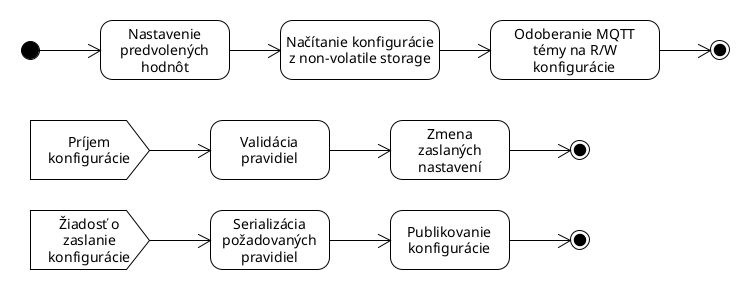
\includegraphics[width=\textwidth]{figures/design/configuration.png}
	\caption{Príjem nových pravidiel a dopytovanie systémovej konfigurácie}
	\label{config-change}
\end{figure}


\subsection{Preskúmané obmeny}
Uvažovalo sa o vložení voliteľného kroku zníženia šumu v transformovanom spektre Welchovou metódou, ktorý by vedel prispieť
k eliminácii záchvevov krátkodobého výpadku frekvenčnej zložky. Nespolupracuje však dobre s ideou zdieľanej veľkosti okna a 
ich prekryvu. Vo všestrannom riešení môžu byť body delené do viacerých segmentov, čo naráža na pamäťové obmedzenia zariadenia
pri viacerých alebo dlhších segmentoch. Zároveň sa znižuje presnosť v časovej oblasti, ktorú by bolo potrebné zohľadniť v časových
pečiatkach udalostí. 

Exploratívnou analýzou sa preukázalo, že v uvažovanom kontexte dopravy nemá zmysel extrahovať zo snímaného zrýchlenia odhad
o rýchlosti a polohe numerickou kvadratúrou korigovanou obálkami, respektíve pre vysoký šum sú hodnoty veličín nerealistické.
Korekciu je uplatniteľná iba pre stacionárne signály vytrácajúce sa v situáciach, keď sa os akcelerácie odchýli medzi 
rovnovážnymi bodmi, napríklad auto zastavené na svahu.

%TODO
\section{Prúdový algoritmus detekcie zmien frekvencií}
Nevidí celý prúd naraz ani ho nemôže celý uložiť. Welchove priemerovanie vyžaduje veľa pamäte pre dlhšie okno.
Ale musíme dosiahnuť odšumenie detegovanie špičiek a zároveň posielať cez sieť menej ako nespracované
frekvenčné vedierka. Detegovanie anomálií, resp. automatické upozornenie na prevládajúce zložky.
Binárna sekvencia

\begin{figure}[h]
\centering
\begin{subfigure}[b]{0.8\textwidth}
    \centering
    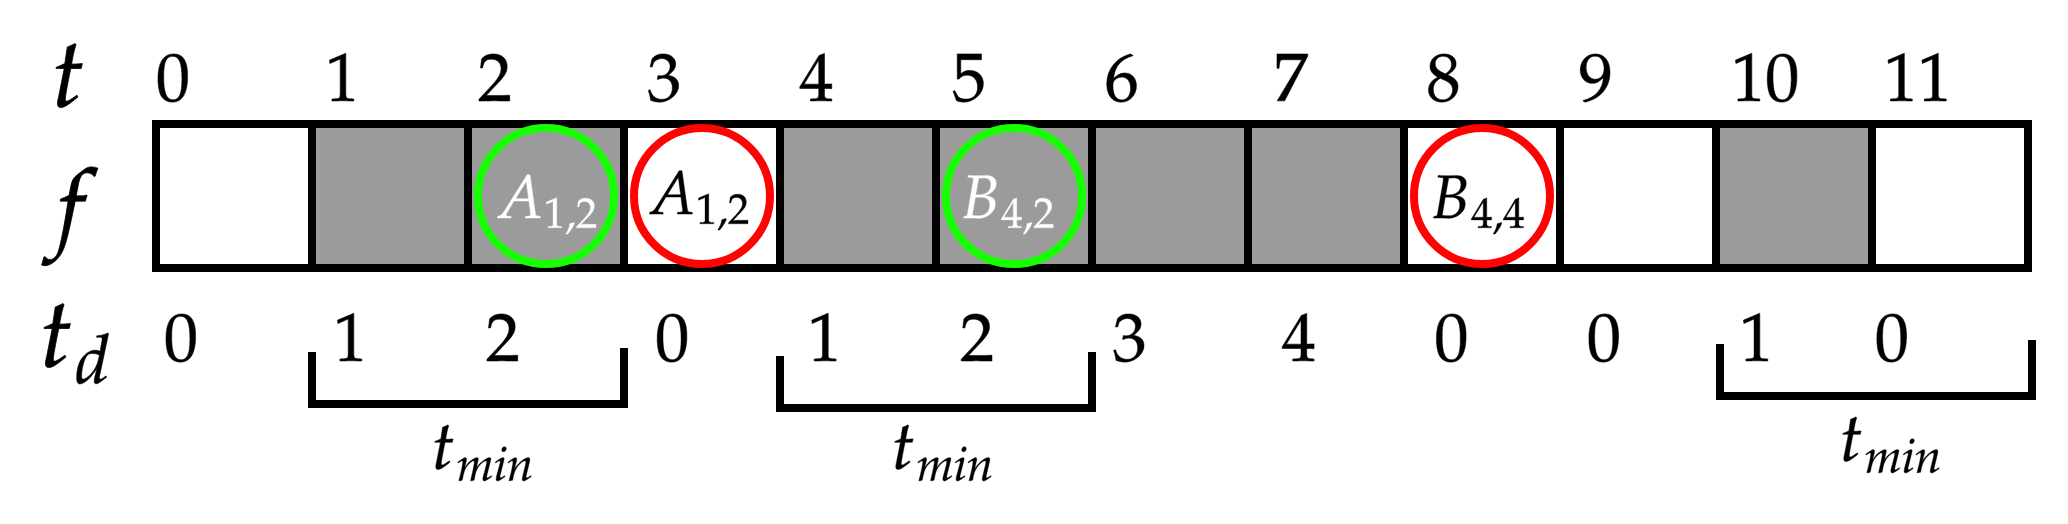
\includegraphics[width=\textwidth]{figures/design/event-detection-min-duration.png}
    \caption{Minimálne trvanie udalosti $t_{\min} = 2$}
\end{subfigure}
\begin{subfigure}[b]{0.8\textwidth}
    \centering
    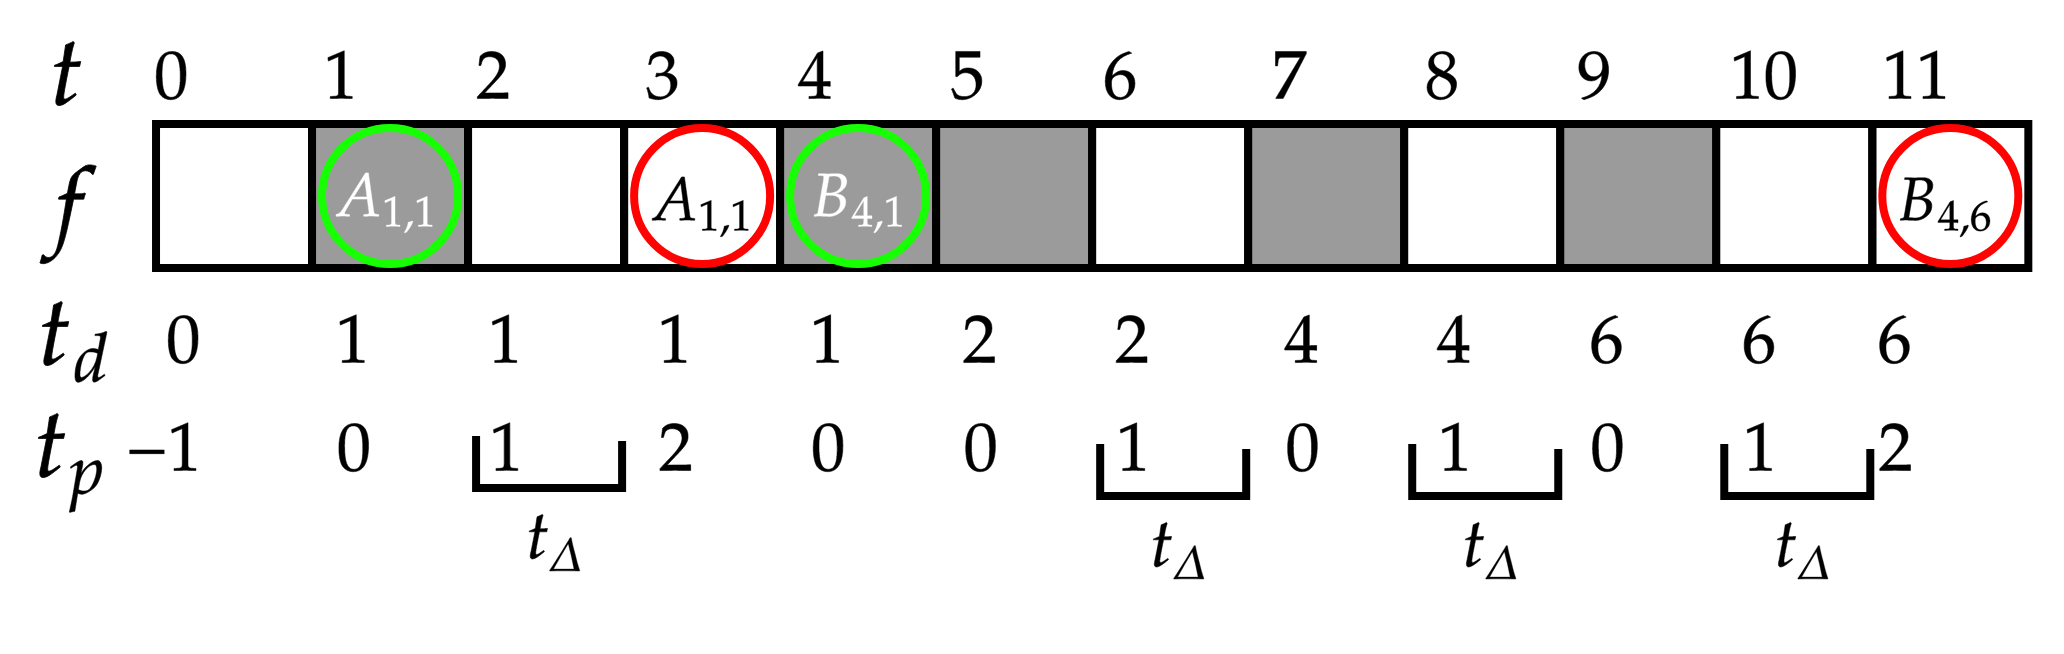
\includegraphics[width=\textwidth]{figures/design/event-detection-time-proximity.png}
    \caption{Maximálna vzdialenosť špičiek $t_{\Delta} = 1$ v čase}
\end{subfigure}
\caption{Parametre algoritmu na detekciu udalostí. $t$ je poradové číslo okna, $f$ je stav detegovanie špičky
vo frekvenčnom vedierku, $t_d$ je trvanie udalosti (duration), $t_p$ je počet okien do minulosti naposledy videnej špičky (past)}
\end{figure}

\begin{algorithm}[h]
\caption{Detektor zmeny frekvenčnej zložky}
\begin{algorithmic}[1]
\Require{$event$, $bin$, $t$, $t_{min}$, $t_{\Delta}$}
\If {V predošlom okne $t - 1$ bola emitovaná udalosť Koniec}
	\State Vynuluj udalosť: $event$: $duration \gets amplitude \gets 0$, $lastSeen \gets -1$
\EndIf

\If {$\mathrm{IsPeak}(bin)$}  
	\State $link \gets \max\{1, event.lastSeen + 1\}$
	\If {$event.duration < t_{min} \leq event.duration + link$}
		\State $event.start \gets t - event.duration - link + 1$
		\State \textbf{Emituj udalosť Štart} výskytu frekvencie podľa $event$
	\EndIf
	
	\State \textbf{Inkrementuj} $event.duration$ \textbf{o} $link$
	\State \textbf{Inkrementuj} $event.amplitude$ \textbf{o} $(bin - event.amplitude)\;/\;event.duration$
	\State $event.lastSeen \gets 0$

\ElsIf {$event.lastSeen \geq 0$}
	\State \textbf{Inkrementuj} $event.lastSeen$ \textbf{o}  $1$

	\If {$events.lastSeen > t_{\Delta}$}
        	\If {$event.duration \geq t_{min}$}
        		\State \textbf{Emituj udalosť Koniec} výskytu frekvencie podľa $event$
        	\EndIf
        \Else
        	\State Vynuluj udalosť: $event$: $duration \gets amplitude \gets 0$, $lastSeen \gets -1$
        \EndIf
\EndIf
\end{algorithmic}
\label{algo:event-detector}
\end{algorithm}

\section{Datasety}
\subsection{Zber vibrácií z premávky}
V časti motora alebo nad nápravou z mestskej hromadnej dopravy. 500Hz, rozlíšní 2g z v režime zapisovania na SD kartu.
Predošlé prieskumné merania na akcelerometri smarfónu ukázali rozsah do +/-$8 m/s^2$do 1g najčastejšie do $2 - 3 m/s^2$

Pre LSB formát je tesne pod teoretickou hranicou rýchlosti UART (115200 baud). 1 znak = 8b + štart + stop = 10bitov.
Rozsah hodnôt signed int16 (5-ciferné číslo a znamienko na jednu súradnicu). Riadok mal teda aj s medzerami a novým riadkom max.
21 znakov na 3D vzorku. 21 znakov je 210 bitov. Teoretická max. vzorkovacia frekvencia je 548 Hz.

Realistické vzhľadom k prevážanému obsahu

\subsection{Generátor frekvenčného spektra}
Opis políčok konfigurácie a postup generovania fade-in/out sinsoid a náhodné vkladanie do signálu

\begin{figure}[h]
   \centering
    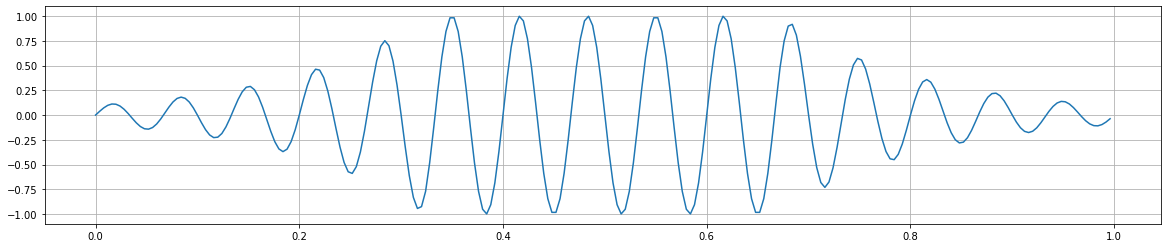
\includegraphics[width=0.8\textwidth]{figures/verification/fade-in-sinusoid.png}
   \caption{Základný tón formujúci syntetický signál}
\end{figure} 
